\documentclass{article}
\usepackage[utf8]{inputenc}
\usepackage{enumitem}
\usepackage[margin=1in]{geometry}
\usepackage{graphicx}
\usepackage{tikz}
\usepackage{authblk}

\begin{document}

% Manually create the title
\noindent
\begin{center}
    \textbf{\LARGE Surgical Room Simulation} \\
    \textit{First phase of simulation assignment} \\
    \vspace{0.5em} % Adjust this value to control spacing
    \textbf{Abdelaziz Ibrahim, Besher Alkurdi, Bishwash Khanal} \\
    TIES481-24 Simulation \\
    University of Jyv\"{a}skyl\"{a} \\
    \today
\end{center}

\section{Overview}
A surgical room facility consisting of one preparation room, one operating theatre, and multiple recovery rooms. The model will be evaluated based on the average 
throughput time for patients and the operating theater blocking time. The average throughput time will be calculated by dividing the total patient time with number of 
patients.

\section{Event-based Model}

\subsection{System Variables and Data Structures}

\subsubsection{System State Variables}
\begin{itemize}
    \item preparation\_facility\_status (busy/available)
    \item operating\_theatre\_status (busy/available)
    \item recovery\_rooms\_status[\hspace{1em}] (array of busy/available states)
    \item blocking\_timer\_status (on/off)
    \item current\_blocking\_time
    \item total\_blocking\_time
    \item total\_number\_of\_patients
    \item total\_patient\_time
\end{itemize}

\subsubsection{Queue Structure}
\begin{itemize}
    \item preparation\_queue
    \item operation\_queue
    \item recovery\_queue
\end{itemize}

\subsubsection{Patient Attributes}
\begin{itemize}
    \item entry\_time
    \item prep\_start\_time
    \item prep\_end\_time
    \item operation\_start\_time
    \item operation\_end\_time
    \item recovery\_start\_time
    \item departure\_time
\end{itemize}

\subsubsection{Time Parameters}
\begin{itemize}
    \item inter\_arrival\_time
    \item preparation\_time
    \item operation\_time
    \item recovery\_time
\end{itemize}

\subsection{Events and Their Behaviors}

\subsubsection{Arrival Event}
A patient from a patients stream arrives with interarrival time. If the preparation queue is not full, we put the patient in the queue. 
If it is full, then the patient is not accepted into the system. Once inside the preparation queue, a timer starts (patient enter time), 
then preparation start event is triggered. Also triggers an arrival event after interarrival time.

\subsubsection{Preparation Start Event}
If the preparation facility is available, pulls a patient from the preparation queue, changes the availability into busy, then triggers 
preparation end event after preparation time.

\subsubsection{Preparation End Event}
Adds the patient to the operation queue, triggers operation start event.

\subsubsection{Preparation Empty Event}
Makes the preparation room available, triggers preparation start event.

\subsubsection{Operation Start Event}
If the operation queue is not empty and the operation room is available, pulls a patient from the queue, triggers preparation empty event, 
changes the operating room availability into busy, then triggers operation end event after operation time.

\subsubsection{Operation End Event}
Adds the patient to the recovery queue, triggers recovery start events.

\subsubsection{Operation Empty Event}
Makes the operation room available, triggers operation start Event.

\subsubsection{Recovery Start Event}
If the recovery queue is not empty and the recovery room is available, pulls a patient from the queue and stops the blocking timer if it is on, 
triggers operation empty event, changes the recovery room availability into busy, then triggers departure Event after recovery time. If the recovery 
room is not available and the queue is not empty, then starts blocking timer.

\subsubsection{Departure Event}
Calculates the total time spent by the patient in the system, makes recovery room available, removes the patient from the system, triggers recovery start event.

\begin{figure}[ht]
    \centering
    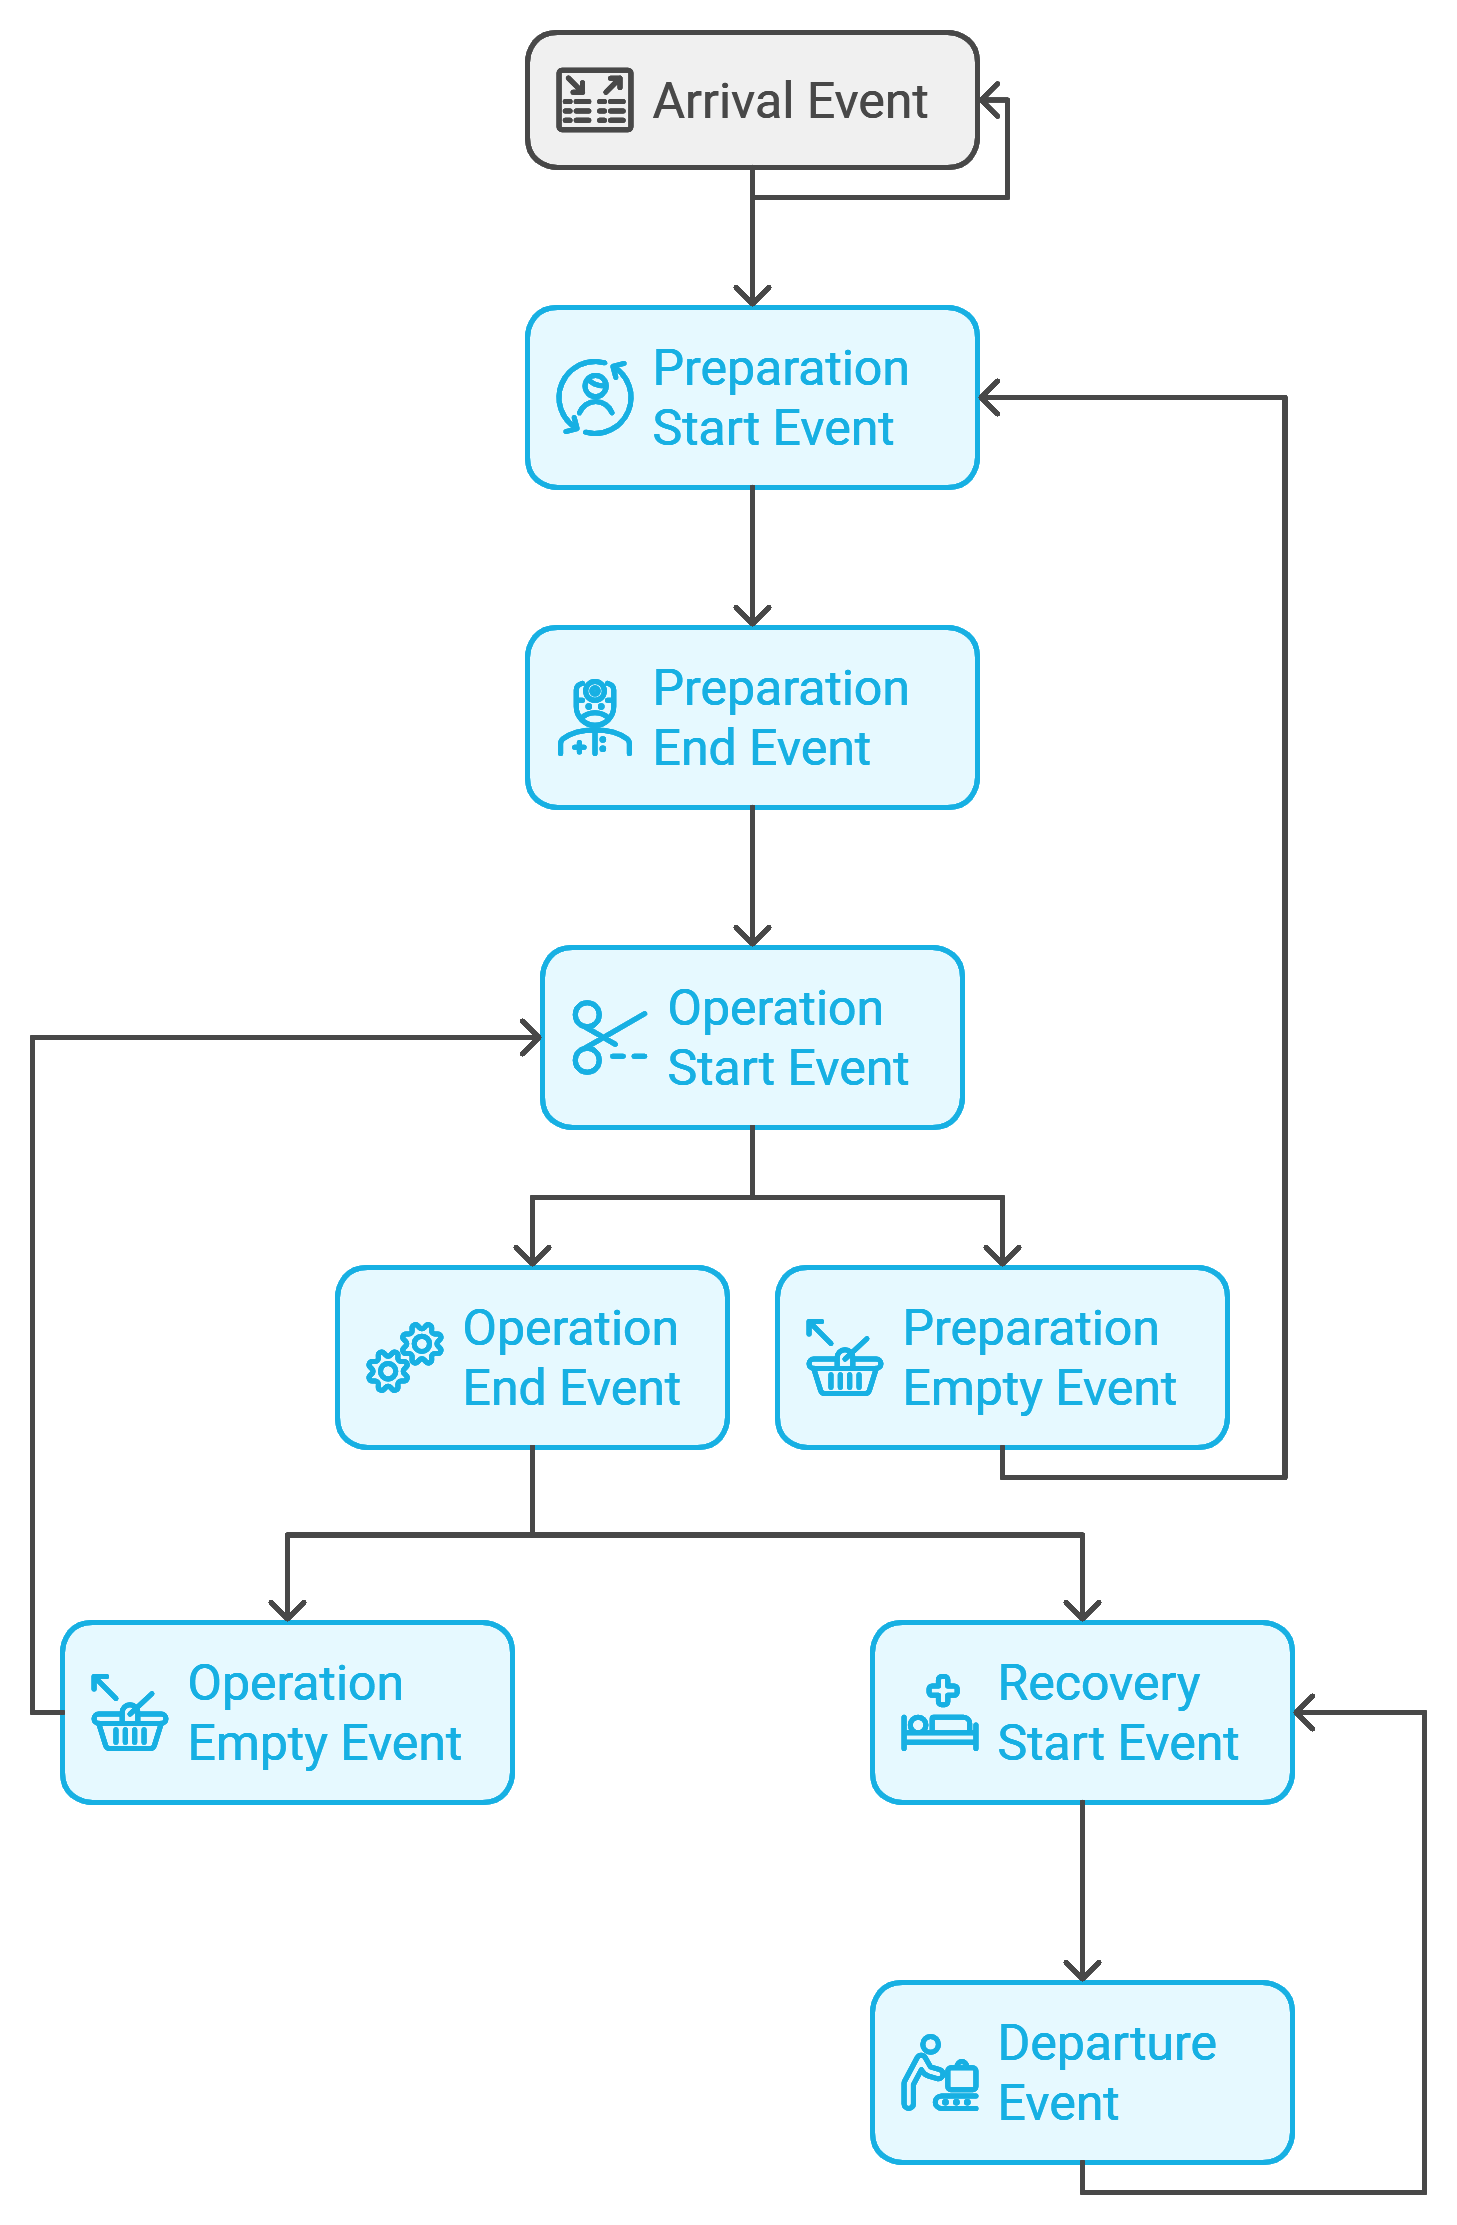
\includegraphics[width=0.4\textwidth]{static/event-based.png}
    \caption{Event-based Flow Diagram for Surgical Room Simulation}
    \label{fig:eventflow}
\end{figure}

\section{Process-based Model}

\subsection{Active Processes}
\begin{itemize}
    \item \textit{PatientGenerator}
    \begin{itemize}
        \item Generates new patient arrivals according to the given inter-arrival time distribution
        \item Activates new Patient processes
    \end{itemize}
    \item \textit{Patient}
    \begin{itemize}
        \item Represents the lifecycle of an individual patient
        \item Manages the patient's journey through preparation, operation, and recovery
        \item Tracks relevant metrics like throughput time and blocking time
    \end{itemize}
\end{itemize}

\subsection{Passive Components}
\begin{itemize}
    \item \textit{PreparationPool}
    \begin{itemize}
        \item Semaphore representing the available preparation facilities
        \item Handles queueing of patients waiting for preparation
    \end{itemize}
    \item \textit{OperatingTheaterPool}
    \begin{itemize}
        \item Semaphore representing the single operating theater
        \item Handles queueing of patients waiting for operation
    \end{itemize}
    \item \textit{RecoveryPool}
    \begin{itemize}
        \item Semaphore representing the available recovery facilities
        \item Handles queueing of patients waiting for recovery
    \end{itemize}
\end{itemize}

The  patient process begins by recording the arrival time. It then tries to request a preparation facility from the PreparationPool. If successful, 
it holds for the preparation time. If not, it waits until a preparation facility becomes available. Next, it tries to request an operating theater 
from the OperatingTheaterPool. If successful, it releases the preparation facility. If not, it waits until an operating theater becomes available. 
It then holds for the operation time. It tries to request a recovery facility from the RecoveryPool. If successful, it releases the operating theater. 
If not, it starts a blocking timer, waits until a recovery facility becomes available, and stops the blocking timer. It then holds for the recovery time, 
releases the recovery facility, records the completion time, and calculates the total time in the system and the blocking time.

\begin{figure}[ht]
    \centering
    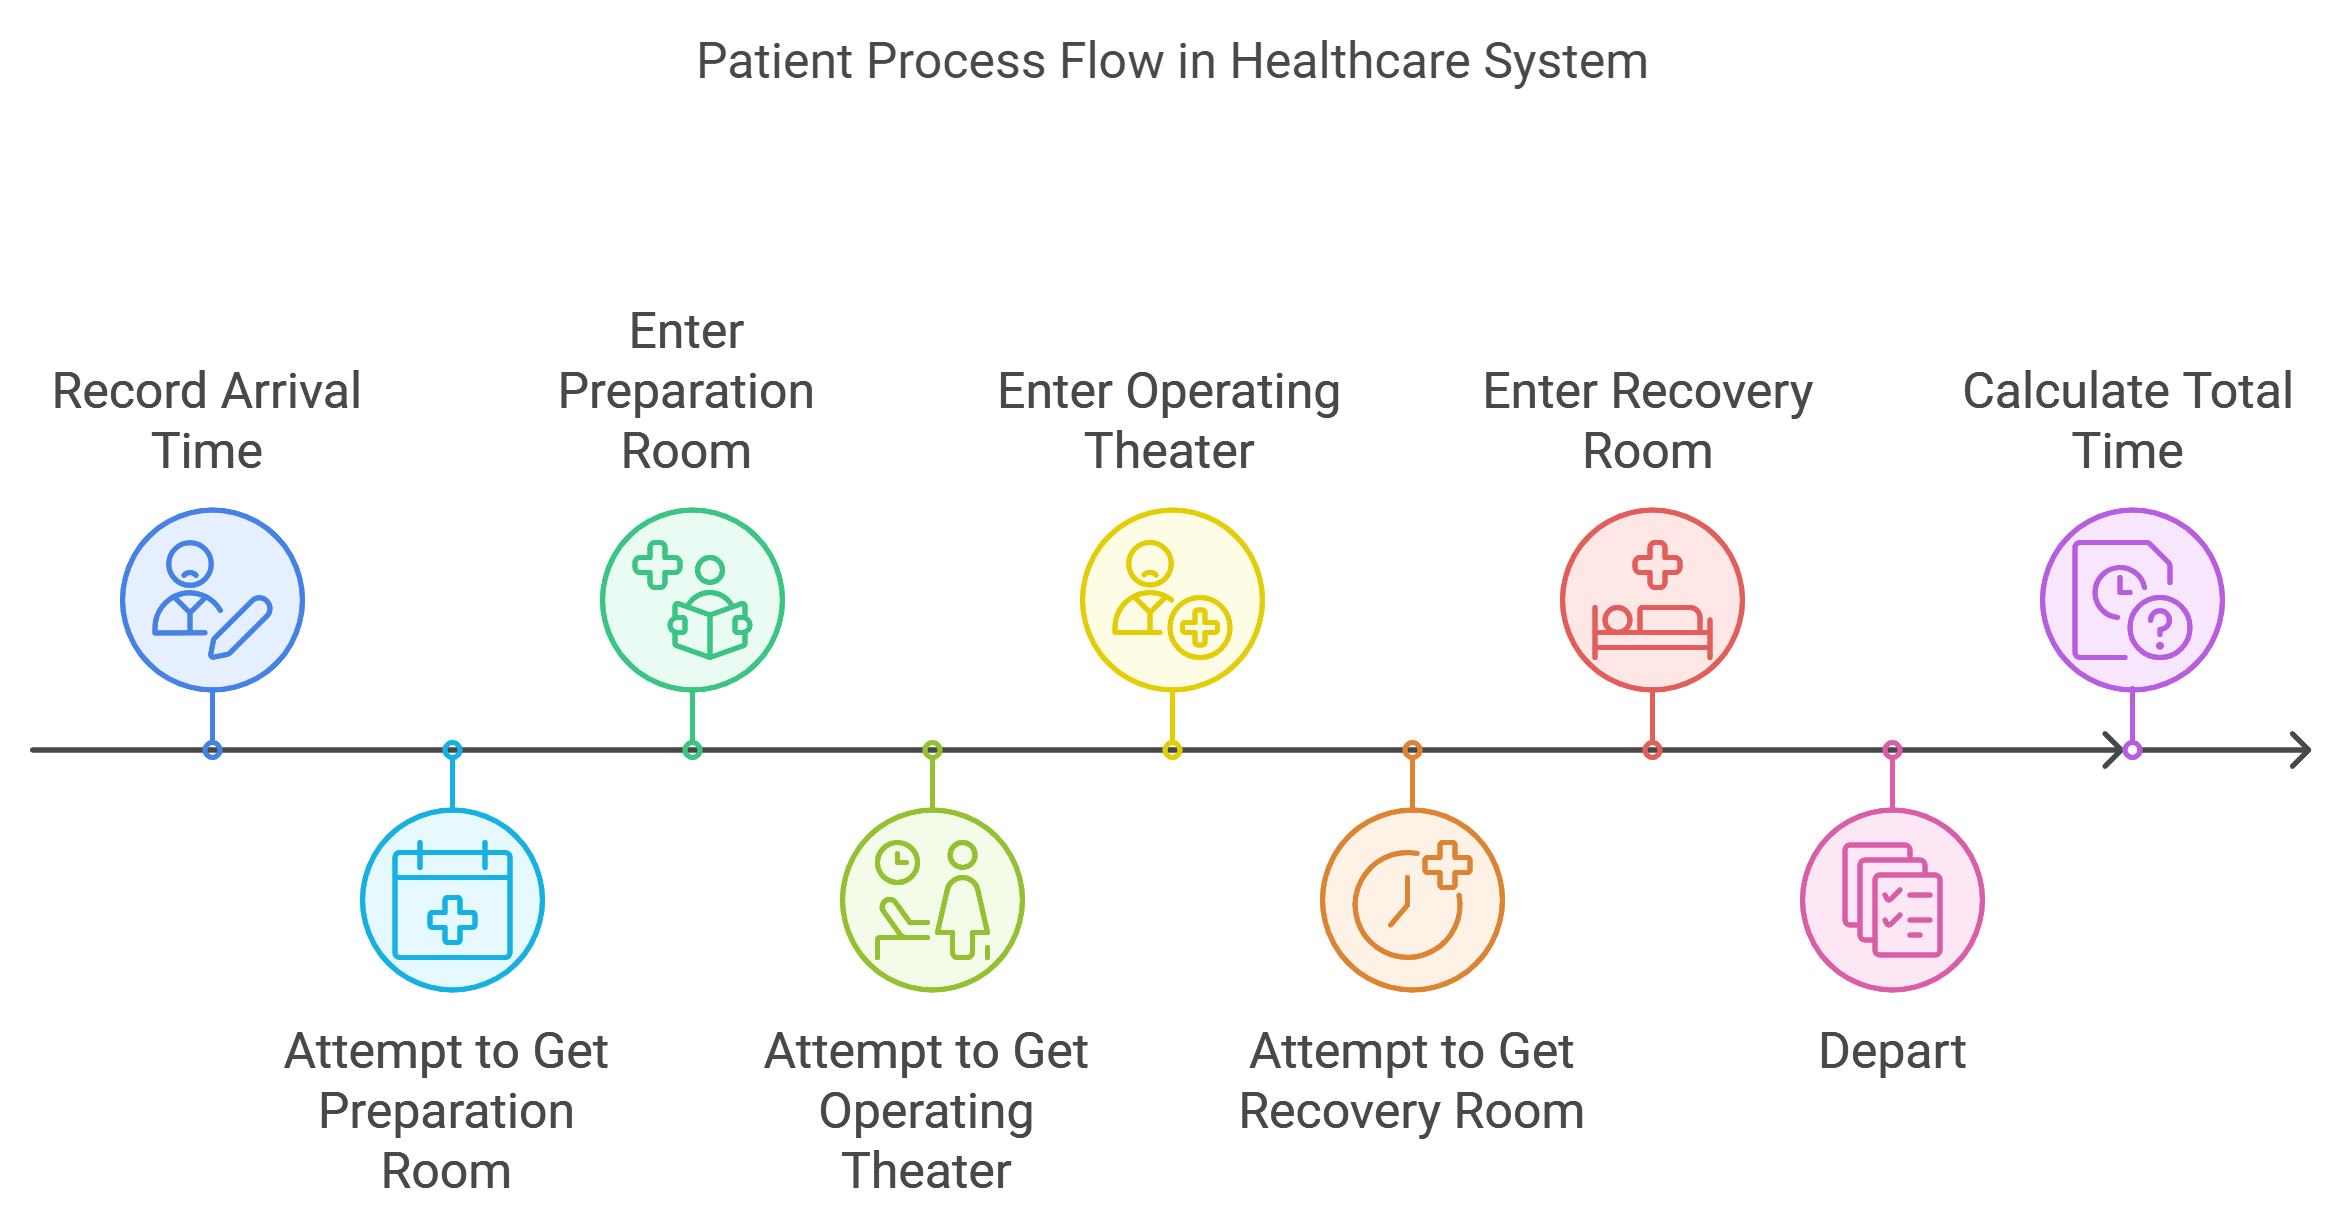
\includegraphics[width=0.6\textwidth]{static/process-based.png}
    \caption{Process-based Flow Diagram for Surgical Room Simulation}
    \label{fig:processflow}
\end{figure}

\subsubsection{Pseudocode}

Below is a pseudocode showing the patient life cycle throughout the process: 

\begin{verbatim}
BEGIN
    Record arrival time
    TRY to REQUEST preparation facility from PreparationPool
    IF successful:
        HOLD for preparation time
    ELSE:
        WAIT until preparation facility becomes available

    TRY to REQUEST operating theater from OperatingTheaterPool:
        IF successful:
            RELEASE preparation facility
        ELSE:
            WAIT until operating theater becomes available

    HOLD for operation time
    TRY to REQUEST recovery facility from RecoveryPool:
        IF successful:
            RELEASE operating theater
        ELSE:
            START blocking timer
            WAIT until recovery facility becomes available
            STOP blocking timer

    HOLD for recovery time
    RELEASE recovery facility
    
    Record completion time
    Calculate total time in system and blocking time
EXIT
\end{verbatim}

\section{Additional Features}

\subsection{Priority Queue}
In addition to the standard patient flow, the simulation can be improved by allowing priority patients like emergency cases. We can do this by implementing a priority 
queue that prioritizes certain patients for operations based on their urgency. This feature will ensure that emergency cases are handled in time.

\subsection{Variable Operations and Patients}
We will have different types of patients based on the operation needed. And the operation will also vary based on properties of probability 
distributions (like mean and standard deviation).

\end{document}